\subsection{Test set primary results}\label{sec:test}
We tested whether spatial information improves fine-grained grading. On the 4,107-image, 240-patient, four-center test set, full VCRE-Fib achieves the lowest prespecified composite risk ($\risk=0.186865$), followed by w/o Weak Loc.\ (0.191308), w/o View (0.193799), and SFibAI (0.201180; Table~\ref{tab:main}). Their respective absolute differences from SFibAI are $-0.014315$, $-0.009872$, and $-0.007380$, corresponding to reductions of 7.115\%, 4.907\%, and 3.668\%, computed before rounding. All spatial variants outperform SFibAI on this endpoint. Results use validation-selected, frozen checkpoints.
\inputtable{tab01_main}

\subsection{Module deletions reveal distinct risk profiles}
Independently trained deletion variants show distinct advantages. The view-retaining w/o Weak Loc.\ has lower patient-max COR, whereas the localization-retaining w/o View has lower image and patient-median COR (Table~\ref{tab:main}). The full model leads all three risks and center-balanced COR, improving composite risk by 0.004443 over the better variant, w/o Weak Loc. Gains thus span risk measures. These design-level comparisons do not isolate supervision, capacity, or information use, or establish statistical superiority or module synergy.

\subsection{Grading gains extend across images and patients}
Specific grading metrics improve alongside composite risk. Relative to SFibAI, full VCRE-Fib reduces image MAE from 0.391313 to 0.377857, increases four-grade accuracy from 64.11\% to 67.03\%, and reduces severe errors from 9.98\% to 9.37\% (Table~\ref{tab:image}). The full model also leads the remaining image metrics: RMSE, TMAE, COR, $\pm0.3$ and $\pm0.5$ accuracy, and macro-F1. The observed gains therefore span score error, agreement within tolerances, and four-grade discrimination.
\inputtable{tab05_image}

The full model also has the lowest patient-max, patient-median, and center-balanced COR (Table~\ref{tab:main}). Some thresholded accuracies favor deletion variants; Appendix~\ref{sec:appendix-patient} reports the complete patient-level metrics and these differences.

\subsection{Lower grading risk accompanies spatial-task trade-offs}
We next examined the accompanying spatial predictions. Full VCRE-Fib reaches view accuracy of 66.81\%, macro-F1 of 0.665861, and CE of 0.916542 on 4,107 test images, with weak-target Dice/IoU of 0.360312/0.235487 on 4,035 eligible images (Table~\ref{tab:auxiliary}). Yet w/o Weak Loc.\ achieves higher view accuracy and macro-F1 (75.70\% and 0.757500), and w/o View achieves higher Dice/IoU (0.430661/0.298825). Thus, the lowest grading risk does not coincide with the best spatial-task scores. Only the full model provides all three outputs, with auxiliary-task trade-offs. Weak-target overlap measures agreement with coarse local annotations, not complete lesion segmentation.
\inputtable{tab07_auxiliary}

\subsection{Joint outputs expose grading--spatial disagreements}
Figure~\ref{fig:cases} illustrates four test cases spanning distinct true views, juxtaposing ultrasound, clinician annotation, and localization with reference/predicted scores and full view names. Rows (a)--(c) show localization correspondence. In (a), scores agree closely (2.4/2.409), yet the true left subcostal transverse view is classified as subxiphoid sagittal. Close score agreement thus need not imply a correct spatial judgment; the joint outputs make this disagreement visible.

Row (d), with scores 1.4/1.491, shows responses outside local rectangles under the fixed scale and threshold; two validation examples appear separately in the appendix. Responses outside annotations offer locations to inspect but may represent relevant tissue or erroneous activation, establishing neither complete lesion coverage nor clinical correctness. All qualitative case predictions were generated with the frozen checkpoint evaluated quantitatively. They illustrate inspectable information, without assigned clinical interpretations or claims of evaluated clinical-review benefit.
\begin{figure}[!tb]
\centering
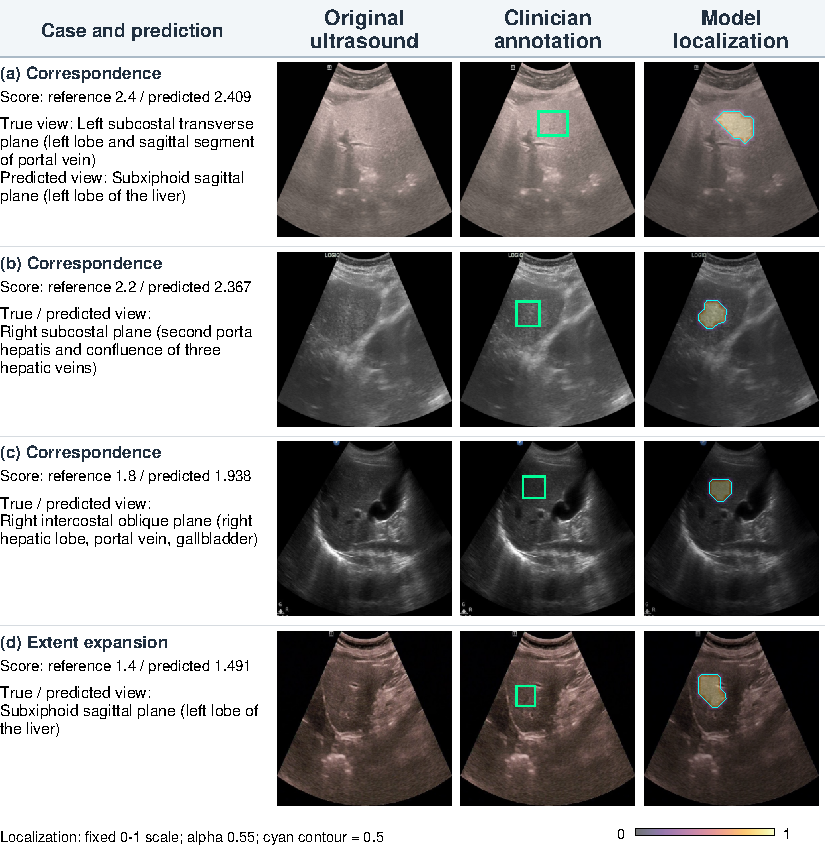
\includegraphics[width=\linewidth]{figures/assets/fig06_cases.pdf}
\caption{\lang{Four selected test cases, with reference and predicted scores and acquisition views at left. Predictions use the frozen checkpoint evaluated quantitatively. Rows (a)--(c) show localization correspondence; (d) shows a response beyond local boxes. Green boxes denote clinician annotations; localization uses a $[0,1]$ scale, opacity 0.55, and a cyan 0.5 contour. In row (a), the predicted view differs from the reference. These selected examples illustrate spatial outputs without establishing population localization performance or complete lesion extent.}{四个筛选的测试集病例，左侧标出参考及预测评分和扫查切面。预测使用参与定量评价的冻结检查点。(a)--(c) 展示定位对应，(d) 展示局部框外响应。绿色框为医生标注；定位色标为 $[0,1]$、透明度为 0.55，青色轮廓阈值为 0.5。(a) 的预测切面与参考切面不同。这些筛选示例用于展示空间输出，不代表总体定位水平或完整病灶范围。}}
\label{fig:cases}
\end{figure}


\subsection{Computational cost of joint prediction}
We quantified the cost of providing grading and both spatial outputs. Matched FP32 measurements on an A100-SXM4-80GB yield median batch-one latencies of 5.620, 6.171, 7.122, and 7.371 ms for SFibAI, w/o View, w/o Weak Loc., and full VCRE-Fib. The full model adds 7.81\% parameters, 4.24\% counted MACs, and 1.751 ms median latency over SFibAI. Appendix Table~\ref{tab:resources} reports latency, P95, and memory at batch sizes one and eight.
